\section{Introduction}
 
\textbf{You can cite books \cite{Feynman1998} and papers \cite{Lee2016} like this, and they appear in the references section toward the end of the document. (Click on the reference number and it will take you there!)}

\lipsum[5-7] % generic text; delete this and replace with your text

\textbf{You can also include and reference figures, for example, see Figure \ref{fig:example}.}
 
\begin{figure}[h]
    \centering
    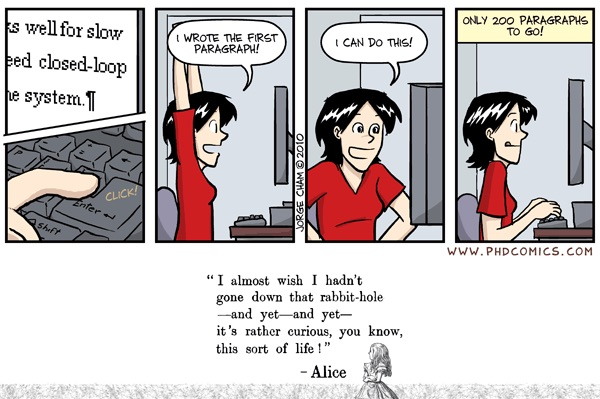
\includegraphics[width=0.9\textwidth]{./images/phd022410s.jpg}
    \caption{Here is a comic from \href{http://phdcomics.com/comics/archive.php?comicid=1285}{PhDComics}. (The previous word is also a clickable link! But if you click it, don't fall down the rabbit hole reading comics rather than writing your essay!). If you get stuck procrastinating, read this article as an antidote: \href{https://www.waitbutwhy.com/2013/10/why-procrastinators-procrastinate.html}{Why procrastinators procrastinate}. }
    \label{fig:example}
\end{figure}

